\chapter{Tipos Abstractos de Datos (TADs o ADTs en inglés)}

Un tipo abstracto de datos (TAD) es una colección de valores y operaciones que se definen mediante una especificación que es independiente de cualquier representación.

Un TAD es una abstracción:
\begin{itemize}
    \item Se destacan los detalles de la especificación (el qué),
    \item Se ocultan los detalles de la implementación (el cómo).
\end{itemize}

\section{Especificación de un TAD}
Para especificar un TAD se deben definir:
\begin{enumerate}
    \item Su \textbf{nombre}.
    \item Especificar \textbf{constructores}: procedimientos o funciones mediante los cuales puedo crear elementos del tipo que estoy especificando.
    \item Especificar \textbf{operaciones}: todos los procedimientos o funciones que permitirán manipular los elementos del tipo de datos que estoy especificando.
    \item Indicamos los \textbf{tipos} de cada constructor y operación (el encabezado de los procedimientos o funciones), y mediante lenguaje natural explicamos qué hacen.
    \item Algunas operaciones pueden tener restricciones que las indicamos mediante \textbf{precondiciones}.
    \item Debemos especificar también una operación de destrucción que libera la memoria utilizada por los elementos del tipo, en caso que sea necesario.
\end{enumerate}

\subsection{Ejemplo}
Suponga que se va a desarrollar un programa para administrar la información de una biblioteca.

Puesto que allí hay elementos como ficheros, usuarios, libros, etc., que participan en el problema, en el software existirá un TAD que represente y simule la operación de cada uno de ellos: el TAD Fichero, el TAD Usuario y el TAD Libro. Estos TAD estarán relacionados dentro del programa, de la misma manera como los elementos que modelan están relacionados en la biblioteca: un elemento del TAD Usuario puede tener en préstamo un elemento del TAD Libro, los elementos del TAD Fichero tienen elementos del TAD Ficha, que representan libros de la biblioteca, etc. No existirá un TAD Pared, puesto que no participa en el problema, así haga parte de la biblioteca (a menos, claro está, que se trate de un sistema de diseño arquitectónico, en el cual las paredes sean los elementos de base.

\section{Implementación de un TAD}
\begin{itemize}
    \item Definir un nuevo tipo con el nombre del TAD especificado. Para ello utilizamos tipos concretos y otros tipos definidos previamente.
    \item Implementar cada constructor respetando los tipos tal como fueron especificados.
    \item Implementar cada operación respetando los tipos tal como fueron especificados.
    \item Implementar operación de destrucción liberando memoria si es que se ha reservado al construir los elementos.
    \item Pueden surgir nuevas restricciones que dependen de cómo implementamos el tipo.
    \item Puedo necesitar operaciones auxiliares que no están especificadas en el tipo.
\end{itemize}

\section{TAD Lista}
Las listas son colecciones 0 o mas elementos de un mismo tipo, de tamaño variable.

\subsection{Especificación}
\begin{itemize}
    \item \textbf{Nombre}: Lista
    \item \textbf{Constructores}:
    \begin{itemize}
        \item \texttt{empty()}: crea una lista vacía. 
\begin{codebox}{Constructores}
\footnotesize empty()
\tcblower
\begin{pascallike}
fun empty() ret l : List of T
{- crea una lista vacia. -}
\end{pascallike}
\end{codebox}
        \item \texttt{addl()}: agrega un elemento al comienzo de la lista.
\begin{codebox}{Constructores}
\footnotesize addl()
\tcblower
\begin{pascallike}
proc addl (in e : T, in/out l : List of T)
{- agrega el elemento e al comienzo de la lista l. -}
\end{pascallike}
\end{codebox}
    \end{itemize}
    \item \textbf{Operaciones}:
    \begin{itemize}
        \item decidir si una lista es vacía,
        \item tomar el primer elemento,
        \item tirar el primer elemento,
        \item agregar un elemento al final,
        \item obtener la cantidad de elementos,
        \item concatenar dos listas,
        \item obtener el elemento en una posición específica,
        \item tomar una cantidad arbitraria de elementos,
        \item tirar una cantidad arbitraria de elementos,
        \item copiar una lista en una nueva.
    \end{itemize}
\end{itemize}

\begin{codebox}{TAD Lista}
\begin{pascallike}
spec List of T where

constructors    
    fun empty() ret l : List of T
    {- crea una lista vacia. -}

    proc addl (in e : T, in/out l : List of T)
    {- agrega el elemento e al comienzo de la lista l. -}

destroy
    proc destroy (in/out l : List of T)
    {- Libera memoria en caso que sea necesario. -}

operations
    fun is_empty(l : List of T) ret b : bool
    {- Devuelve True si l es vacia. -}

    fun head(l : List of T) ret e : T
    {- Devuelve el primer elemento de la lista l -}

    {- PRE: not is_empty(l) -}
    proc tail(in/out l : List of T)
    {- Elimina el primer elemento de la lista l -}

    {- PRE: not is_empty(l) -}
    proc addr (in/out l : List of T,in e : T)
    {- agrega el elemento e al final de la lista l. -}

    fun length(l : List of T) ret n : nat
    {- Devuelve la cantidad de elementos de la lista l -}

    proc concat(in/out l : List of T,in l0 : List of T)
    {- Agrega al final de l todos los elementos de l0
    en el mismo orden.-}

    fun index(l : List of T,n : nat) ret e : T
    {- Devuelve el n-esimo elemento de la lista l -}

    {- PRE: length(l) > n -}
    proc take(in/out l : List of T,in n : nat)
    {- Deja en l so lo los primeros n
    elementos, eliminando el resto -}

    proc drop(in/out l : List of T,in n : nat)
    {- Elimina los primeros n elementos de l -}

    fun copy_list(l1 : List of T) ret l2 : List of T
    {- Copia todos los elementos de l1 en la nueva lista l2 -}
\end{pascallike}
\end{codebox}

\subsection{Ejempo de uso}

\begin{codebox}{Promedio}
\footnotesize Uso de operaciones de listas
\tcblower
\begin{pascallike}
fun promedio (l : List of float) ret r : float
    var largo : nat
    var elem : float
    var laux : List of float

    laux := copy(l) {- copio la lista para no modificar la original -}
    r := 0.0 {- inicializo el promedio en 0 -}
    largo := length(laux) {- obtengo la cantidad de elementos -}
    do (not is_empty(laux)) -> {- mientras la lista no sea vacia -}
        elem := head(laux) {- tomo el primer elemento -}
        r := r + elem {- sumo el elemento al promedio -}
        tail(laux) {- elimino el primer elemento -}
    od
    destroy(laux) {- libero la memoria -}
    r := r / largo {- calculo el promedio -}
end proc
\end{pascallike}
\end{codebox}

\section{Implementación de un TAD Lista mediante punteros}
\begin{itemize}
    \item Implementaremos el TAD lista utilizando punteros, implementación conocida como \texttt{lista enlazada}.
    \item Cada elemento de la lista estará alojado en un nodo conteniendo además un puntero hacia el siguiente.
    \begin{figure}[h]
        \centering
        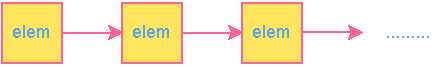
\includegraphics[scale=1]{./estáticos/node.pdf}
        \caption{Lista enlazada}
        \label{fig:my_label}
    \end{figure}
    \item Una lista será un puntero a un nodo.
    \item La lista vacía se implementa con el puntero null.
    \item Esta implementación permite tener la lista de elementos almacenada en lugares de la memoria no necesariamente contiguos.
    \item No existe límite teórico para almacenar elementos. En la práctica dicho límite será la cantidad de memoria.    
\end{itemize}

En resumen, la implementación de un TAD lista mediante punteros consiste en:
\begin{itemize}
    \item Definir un tipo nodo que contenga un elemento y un puntero al siguiente nodo.
    \item Definir un tipo lista que sea un puntero a un nodo.
    \item Implementar cada constructor y operación respetando los tipos especificados.
    \item Implementar la operación de destrucción liberando la memoria utilizada.
\end{itemize}

\textit{La implementación completa del TAD lista mediante punteros se encuentra en el solucionario.}

\section{TAD Contador}
Un problema interesante (y no del todo trivial) es el de controlar que una cierta expresión tiene balanceados sus paréntesis. Se quiere dar un algoritmo que tome una expresión (dada, por ejemplo, por un arreglo de caracteres) y devuelva verdadero si la expresión tiene sus paréntesis correctamente balanceados, y falso en caso contrario.
Este problema puede solucionarse con un algoritmo que recorre la expresión de izquierda a derecha y que utiliza un entero, que se inicializa en 0 y se incrementa cada vez que se encuentra un paréntesis que abre y se decrementa (chequeando previamente que dicho número no sea nulo) cada vez que se encuentra un paréntesis que cierra. Al analizar, sólo resta comprobar que dicho entero sea cero. Esta descripción debería alcanzar para darse uno cuenta de que no es en realidad un entero lo que hace falta, sino mucho menos. Un entero es un objeto que admite todas las operaciones aritméticas, acá sólo se necesita inicializar en 0, incrementar, decrementar y controlar si su valor es o no cero.

\subsection{Especificación}
Los \textbf{constructores} (en este caso inicial e incrementar) deben ser capaces de generar todos los valores posibles del TAD. En lo posible cada valor debe poder generarse de manera única. Intuitivamente, esto se cumple para inicial e incrementar: partiendo del valor inicial y tras sucesivos incrementos se puede alcanzar cualquier valor posible; y hay una única forma de alcanzar cada valor posible de esa manera.

Las demás \textbf{operaciones} quedan declaradas simplemente como tales. Las operaciones se definen con ecuaciones que deben cubrir todos los casos posibles, salvo los declarados que no pueden ocurrir, como en el caso de decrementar que no puede aplicarse a un contador que sea inicial (a pesar de que se podría defnir de manera obvia para ese caso). 
\begin{itemize}
    \item comprobar si su valor es el inicial
    \item decrementar si no lo es
\end{itemize}

\begin{codebox}{TAD Contador}
\begin{pascallike}
spec Counter where

constructors
    fun init() ret c : Counter
    {- crea un contador con valor inicial -}

    proc incr(in/out c : Counter)
    {- incrementa el valor del contador c -}

destroy
    proc destroy(in/out c : Counter)
    {- Libera memoria en caso que sea necesario. -}

operations
    fun is_init(c : Counter) ret b : bool
    {- Devuelve True si el contador c tiene el valor inicial -}

    {- PRE: not is_init(c) -}
    proc decr(in/out c : Counter)
    {- decrementa el valor del contador c -}
\end{pascallike}
\end{codebox}

\subsection{Implementación}

\begin{codebox}{Implementación del TAD Contador}
\begin{pascallike}
implement Counter where
type Counter = nat

proc init (out c: Counter)
    c:= 0
end proc

proc inc (in/out c: Counter)
    c:= c+1
end proc

fun is_init (c: Counter) ret b: bool
    b:= (c = 0)
end fun

{- PRE: not is_init(c) -}
proc dec (in/out c: Counter)
    c:= c-1
end proc

proc destroy (in/out c: Counter)
    skip
end proc
\end{pascallike}
\end{codebox}

\subsection{Algoritmo de balanceo de paréntesis}

\begin{codebox}{Algoritmo de balanceo de paréntesis}
\begin{pascallike}
fun matching_parenthesis (a: array[1..n] of char) ret b: bool
    var i: nat
    var c: Counter
    b:= true
    init(c)
    i:= 1
    do i $\leq$ n $\wedge$ b $\rightarrow$ if a[i] = '(' $\rightarrow$ inc(c)
                                    a[i] = ')' $\wedge$ is_init(c) $\rightarrow$ b:= false
                                    a[i] = ')' $\wedge$ $\neg$is_init(c) $\rightarrow$ dec(c)
                                    otherwise $\rightarrow$ skip
                                fi
                                i:= i+1
    od
    b:= b $\wedge$ is_init(c)
    destroy(c)
end fun
\end{pascallike}
\end{codebox}

\section{TAD Pila}